\subsubsection{Example}

    \begin{itemize}[noitemsep,topsep=0pt]
      \item Starting position: (-9.0, -23.0, 48.0)
      \item End position: (6.0, 3.0, 8.0) 
      \item Euclidean distance from the object: 10.44030650891055
      \item Object can be seen: True
      \item Success: True
      \item Object type: a large trash pile
      
    \end{itemize}
    

    \begin{center}
    \includegraphics[width=0.7\linewidth]{images/GPT4o-CityNew/28_r0_.pdf}
    \end{center}
    

    \begin{center}
    \includegraphics[width=0.7\linewidth]{images/GPT4o-CityNew/28_r0__sit_awareness.pdf}
    \end{center}
    

    \begin{drama}
    \Character{Benchmark}{re}
    \Character{GPT-4o}{gpt}
    
\respeaks: \( < \)Context\( > \)
    You are in command of a UAV, tasked with finding a large trash pile.
\( < \)/Context\( > \) \texttt{(REST OF THE PROMPT)}
\StageDir{\re{} presents \gpt{} with a relevant image}

    \begin{center}
    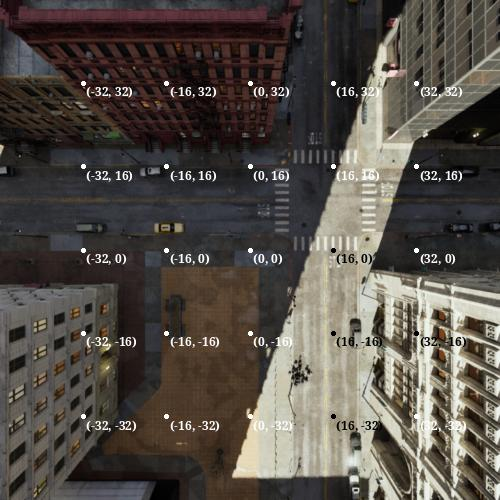
\includegraphics[width=0.5\linewidth]{images/GPT4o-CityNew/28_r0__0.jpg}
    \end{center}
    
\respeaks: Your current altitude is 48 meters above ground level.
\gptspeaks: \( < \)Reasoning\( > \)
The trash pile is not visible in the current field of view. I will start by moving south to get a better view of the area below. I'll also decrease the altitude to get closer to the ground, which will help in identifying the trash pile.
\( < \)/Reasoning\( > \)
\( < \)Action\( > \)(0, -32, -20)\( < \)/Action\( > \)
\StageDir{\re{} presents \gpt{} with a relevant image}

    \begin{center}
    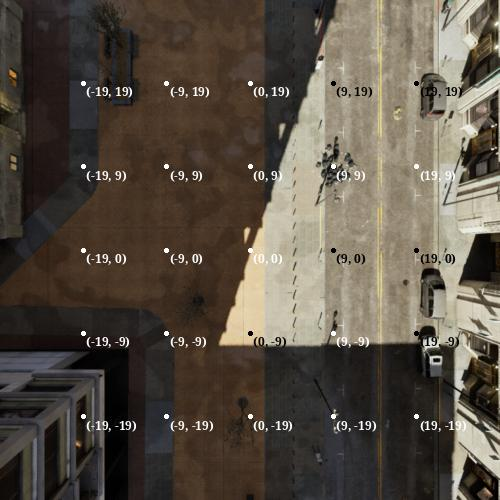
\includegraphics[width=0.5\linewidth]{images/GPT4o-CityNew/28_r0__1.jpg}
    \end{center}
    
\respeaks: Your current altitude is 28 meters above ground level.
\gptspeaks: \( < \)Reasoning\( > \)
The trash pile is not visible yet. I will move slightly east and lower the altitude to improve visibility and continue searching for the trash pile.
\( < \)/Reasoning\( > \)
\( < \)Action\( > \)(9, 0, -10)\( < \)/Action\( > \)
\StageDir{\re{} presents \gpt{} with a relevant image}

    \begin{center}
    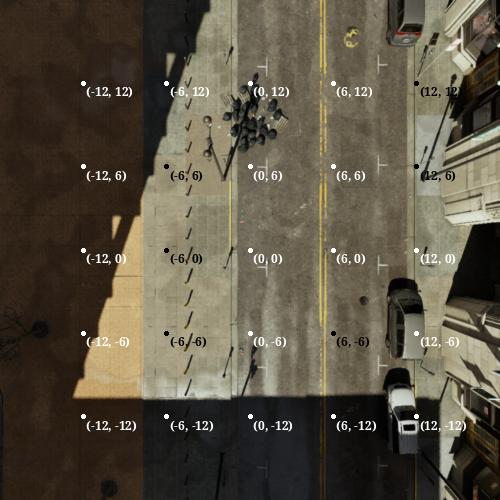
\includegraphics[width=0.5\linewidth]{images/GPT4o-CityNew/28_r0__2.jpg}
    \end{center}
    
\respeaks: Your current altitude is 18 meters above ground level.
\gptspeaks: \( < \)Reasoning\( > \)
There is a pile of objects slightly northeast, which might be the trash pile. I will move closer and lower the altitude to inspect it more closely.
\( < \)/Reasoning\( > \)
\( < \)Action\( > \)(6, 6, -10)\( < \)/Action\( > \)
\StageDir{\re{} presents \gpt{} with a relevant image}

    \begin{center}
    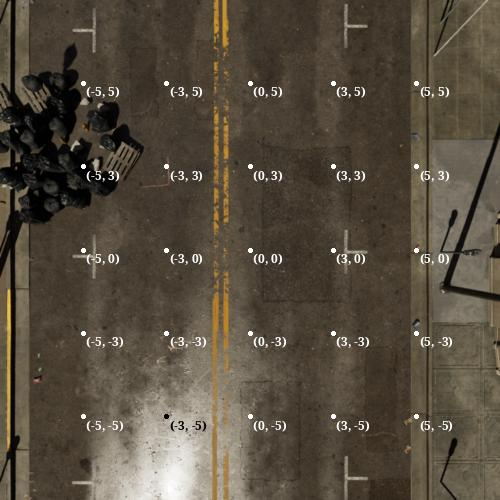
\includegraphics[width=0.5\linewidth]{images/GPT4o-CityNew/28_r0__3.jpg}
    \end{center}
    
\respeaks: Your current altitude is 8 meters above ground level.
\gptspeaks: \( < \)Reasoning\( > \)
The trash pile is clearly visible and centered in the view. I'm now at an altitude of 8 meters, which is below the required 10 meters. I will confirm the find.
\( < \)/Reasoning\( > \)
\( < \)Action\( > \)FOUND\( < \)/Action\( > \)
\end{drama}
\subsubsection{Example}

    \begin{itemize}[noitemsep,topsep=0pt]
      \item Starting position: (0.0, -1.0, 35.0)
      \item End position: (0.0, -1.0, 8.0) 
      \item Euclidean distance from the object: 8.06225774829855
      \item Object can be seen: True
      \item Success: True
      \item Object type: a blue sport car
      
    \end{itemize}
    

    \begin{center}
    \includegraphics[width=0.7\linewidth]{images/GPT4o-CityNew/29_r0_.pdf}
    \end{center}
    

    \begin{center}
    \includegraphics[width=0.7\linewidth]{images/GPT4o-CityNew/29_r0__sit_awareness.pdf}
    \end{center}
    

    \begin{drama}
    \Character{Benchmark}{re}
    \Character{GPT-4o}{gpt}
    
\respeaks: \( < \)Context\( > \)
    You are in command of a UAV, tasked with finding a blue sport car.
\( < \)/Context\( > \) \texttt{(REST OF THE PROMPT)}
\StageDir{\re{} presents \gpt{} with a relevant image}

    \begin{center}
    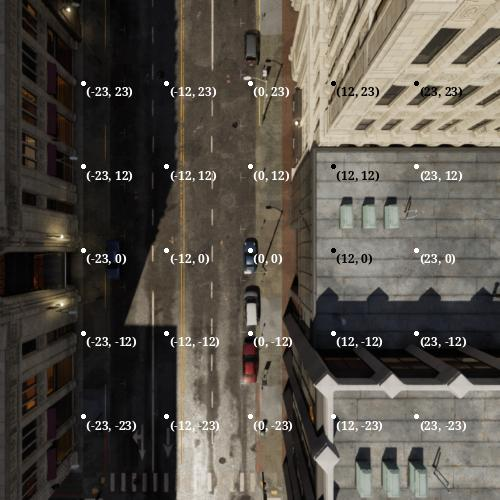
\includegraphics[width=0.5\linewidth]{images/GPT4o-CityNew/29_r0__0.jpg}
    \end{center}
    
\respeaks: Your current altitude is 35 meters above ground level.
\gptspeaks: \( < \)Reasoning\( > \)The blue car is visible at the center of the grid. I need to descend to be within 10 meters above it to confirm the sighting.\( < \)/Reasoning\( > \)
\( < \)Action\( > \)(0, 0, -27)\( < \)/Action\( > \)
\StageDir{\re{} presents \gpt{} with a relevant image}

    \begin{center}
    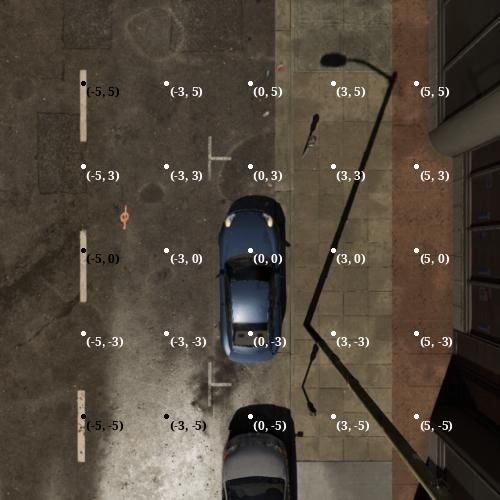
\includegraphics[width=0.5\linewidth]{images/GPT4o-CityNew/29_r0__1.jpg}
    \end{center}
    
\respeaks: Your current altitude is 8 meters above ground level.
\gptspeaks: FOUND
\end{drama}
